% to change the appearance of the header, questions, problems or subproblems, see the homework.cls file or
% override the \Problem, \Subproblem, \question or \printtitle commands.

% The hidequestions option hides the questions. Remove it to print the questions in the text.

\title{MAC4722 - Lista 4}

\documentclass{homework}

\usepackage[utf8]{inputenc}
\usepackage{tikz}
\usetikzlibrary{automata,positioning}

\usepackage{graphicx}
\graphicspath{ {images/} }

% Set up your name, the course name and the homework set number.
\homeworksetup{
    username={Jean Fobe, N$^o$USP 7630573},
    course={Linguagens, Autômatos e Computabilidade - MAC4722},
    setnumber=4}
\begin{document}% this also prints the header.
\pagestyle{fancy}
\fancyfoot[L]{Jean Fobe, 7630573}

% use starred problems or subproblems to apply manual numbering.
\problem*{1}
\question{Seja $L \subseteq \Sigma^*$  uma linguagem regular.  Mostre que $L ^R$ também é regular, descrevendo como construir um autômato finito não determinístico para reconhecer $L^R$
, a partir de um autômato finito (determinístico ou não determinístico)
que reconhece $L$.}\\

	$Resp:$ Queremos mostrar que se $L$ é regular então $L^R$ também é regular.\\
	Seja $A = (Q_A,\Sigma_A,\delta_A,q_A,F_A)$ um autômato finito não determinístico satisfazendo $L = L(A)$. O autômato finito não determinístico $A^R$ definido abaixo aceita a linguagem $L^R$.
	\begin{enumerate}
		\item $A^R = (Q_A \cup \{q_s\},\Sigma_A,\delta_{A^R},q_s,\{q_A\})$, com $q_s \notin Q_A$;
		\item $p \in \delta_A(q,a) \iff q \in \delta_{A^R}(p,a)$, onde $a \in \Sigma_A$ e $p,q \in Q_A$;
		\item Há $\lambda$-transições de $q_s$ para todos elementos de $F_A$.
	\end{enumerate}
	Com isso precisamos provar que existe uma sequencia de transições de q para p que é uma computação da palavra $\omega$ em $A$, se e somente se, existe uma computação de $\omega^R$ em $A^R$ de p para q, com $q,p \in Q_A$. A prova será feita por indução no comprimento de $\omega$.
	\begin{itemize}
		\item Caso Base: Vale $|\omega|=1$ por $\delta_{A^R}$.
		\item Hipótese: Se existe $\omega$ aceito por A e $|\omega|=n,n > 1$, então existe $\omega^R$ aceito por $A^R$.
		\item Passo indutivo: Seja $\omega = xa, a \in \Sigma_A$ e $(r_0,...,r_n)$ a computação de $\omega$ por A. Temos que $p \in \delta(q, r_{n}) = \delta(q, a)$.\\
		Sabendo que $|a| < |x| < n$, pela hipótese de indução temos $p' \in \delta_{A^R}(p,a)$ e $q \in \delta_{A^R}(p', r_0)$. Isso implica em $q \in \delta_{A^R}(p,r_0) \iff p \in \delta_A(q,a)$.\\
		Com $q = q_A$ e $p = s, s \in F_A$, substituindo $\omega^R$ por $ax^R$ garante que $p \in \delta_{A^R}(s, r_0)$. Como há transições vazias de $q_s$ para todos estados de $F_A$ e uma transição de todo estado de $F_A$ para o estado $q_A$, então temos uma computação de $\lambda \omega^R = \omega^R$ começando em $q_s$ e acabando em $q_A$.				
	\end{itemize}


\problem*{2}
\question{Seja $\Sigma_3 = \left \{
				\begin{bmatrix} 0 \\ 0 \\ 0 \end{bmatrix},
				\begin{bmatrix} 0 \\ 0 \\ 1 \end{bmatrix},
				\begin{bmatrix} 0 \\ 1 \\ 0 \end{bmatrix},\ ...\ ,
				\begin{bmatrix} 1 \\ 1 \\ 1 \end{bmatrix}
				\right \}$.\\
		 $\Sigma_3$ contém todas as colunas de tamanho 3 formadas de 0s e 1s. Uma palavra de símbolos de $\Sigma_3$ é composta de 3 linhas de '0's e '1's. Considere cada linha como um número binário e seja $L = \{\omega \in \Sigma^3 :$ a terceira linha de $\omega$ é a soma das suas duas primeiras linhas $\}$.\\
		 Por exemplo,\\
		 \begin{changemargin}{1cm}{1cm} 
		 	$\begin{bmatrix} 0 \\ 0 \\ 1 \end{bmatrix}
		  	\begin{bmatrix} 1 \\ 0 \\ 0 \end{bmatrix}
		  	\begin{bmatrix} 1 \\ 1 \\ 0 \end{bmatrix} \in L, \quad mas \quad 
		  	\begin{bmatrix} 0 \\ 0 \\ 1 \end{bmatrix}
		  	\begin{bmatrix} 1 \\ 0 \\ 1 \end{bmatrix} \not\in L$
		 \end{changemargin}
		 Mostre que L é uma linguagem regular.\\
		 (Sugestão: Mostre que $L^R$ é uma linguagem regular. Depois, utilize o resultado do exercício anterior.)}
	
	$Resp:$	Vamos construir um atômato não determinístico $N, L(N)=L^R$. Para simplificar, vamos representar os símbolos do alfabeto $\Sigma_3$ como triplas ($\Sigma_3 = (0,0,0),(0,0,1),...,(1,1,1)$). Teremos $N = (Q,\Sigma_3,\delta,q_0,F)$:
	
	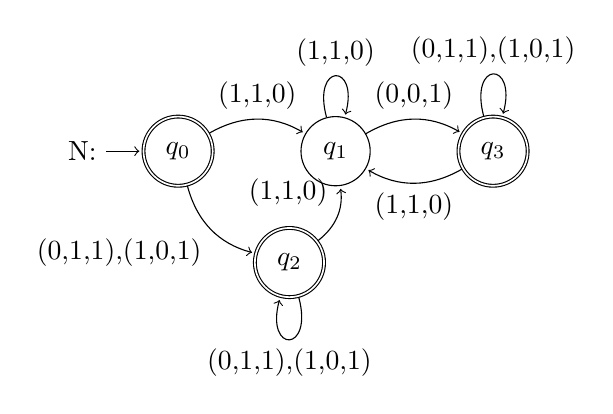
\begin{tikzpicture}[shorten >=1pt,node distance=2cm,on grid,auto,initial text=N:] 
    	\node[state,initial,accepting] (q_0)   {$q_0$}; 
    	\node[state] (q_1) [right=of q_0] {$q_1$}; 
  		\node[state,accepting] (q_2) [below right=of q_0] {$q_2$};
    	\node[state,accepting] (q_3) [right=of q_1] {$q_3$};
        \path[->] 
        (q_0) edge [bend right] node [swap] {(0,1,1),(1,0,1)} (q_2)
              edge [bend left] node {(1,1,0)} (q_1)
        (q_2) edge [bend right] node {(1,1,0)} (q_1)
        	  edge [loop below] node {(0,1,1),(1,0,1)} ()
        (q_1) edge [bend left] node {(0,0,1)} (q_3)
          	  edge [loop above] node {(1,1,0)} ()
        (q_3) edge [bend left] node {(1,1,0)} (q_1)
        	  edge [loop above] node {(0,1,1),(1,0,1)} ()
              ;
	\end{tikzpicture}\\
	Como N descreve $L^R$ e o conjunto de linguagens regulares é fechado para operação de reverso, então $L = (L^R)^R$ é regular.
\problem*{3}
\question{Seja L uma linguagem qualquer sobre $\Sigma$. Definimos $Remove(L)$ como
sendo a linguagem contendo todas as palavras que podem ser obtidas pela remoção
de um símbolo de uma palavra em L. Assim, $Remove(L) = \{xy : x \sigma y \in L,$ onde $x, y \in \Sigma^*$ e $\sigma \in \Sigma \}$. Mostre que a classe de linguagens regulares é fechada sob a operação
$Remove$.}

	$Resp:$	Queremos provar que se $L$ é regular, então $Remove(L)$ também é regular (Página 90 do Sipser, exercício 43).\\
	Se $L$ é regular então existe um autômato $A,L(A)=L$. Seja $A = (Q_A,\Sigma,\delta_A,q_A,F_A)$ o autômato que reconhece $L$. Agora vamos tentar construir um autômato finito não determinístico $N = (Q,\Sigma,\delta,q_0,F)$ que reconhece $Remove(L)$. Trabalharemos com duas 'replicas' do autômato $A$, uma para reconhecer o prefixo antes do símbolo e outra para o sufixo depois do símbolo a ser removido.
	\begin{enumerate}
		\item $Q = Q_A$, os estados de $N$ são os mesmos de $A$;
		\item O estado $q_0 = q_A$ é o estado inicial de $N$;
		\item Os estados de aceitação de $N$ são $F = F_{A'}$ ($A'$ é a 'replica' do autômato $A$ para o sufixo depois do símbolo);
		\item Definimos $\delta$ para quaisqueres $q \in Q$ e $a \in \Sigma$:\\
		$\delta(q,a) = \begin{cases}
							\delta_A(q,a),\qquad q \in Q_A \ e \ a \neq \lambda;\\
							\{q_{A'}\},\qquad q = q_0 \ e \ a = \lambda;\\
							\delta_{A'}(q,a), \qquad  a = \lambda;
					   \end{cases}					  
		$
	\end{enumerate}

	Denotando a construção:
	\begin{enumerate}
		\item Seja $A'$ a replica de $A$; 
		\item Sejam $q_A,..., q_n$ os estados de $A$, então renomeie os estados em $A'$ como $(q_A',..., q_n'$);
		\item Para cada transição: $(\delta(q,a))$ em $A$, fazer uma nova transição $(\delta(q,\lambda))$ para $A'$ (equivalente ao que seria o próximo estado em $A$, ou seja 'pulando' uma transição em $A$ para $A'$). 
		\item O autômato N é formado por $A$ e $A'$ mais as $\lambda$-transições de '3.', com o estado inicial de $N$ seno o estado inicial de $A$.	
	\end{enumerate}
	Exemplo: $A = (Q_A=\{q_A,q_1,q_2\},\Sigma=\{a,b\},\delta_A,q_A,F_A=\{q_2\})$\\
	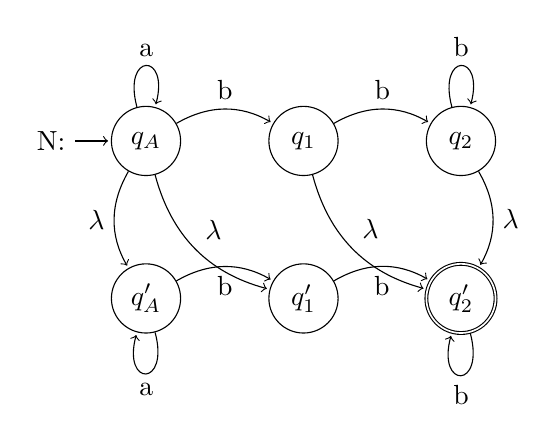
\begin{tikzpicture}[shorten >=1pt,node distance=2cm,on grid,auto,initial text=N:] 
    	\node[state,initial] (q_A)   {$q_A$}; 
    	\node[state] (q_1) [right=of q_A] {$q_1$}; 
    \node[state] (q_2) [right=of q_1] {$q_2$};
    \node[state] (q_A') [below=of q_A] {$q_A'$};
    \node[state] (q_1') [below=of q_1] {$q_1'$};
    \node[state,accepting] (q_2') [below=of q_2] {$q_2'$};
        \path[->] 
        (q_A) edge [loop above] node {a} ()
              edge [bend right] node [swap] {$\lambda$} (q_A')
              edge [bend right] node {$\lambda$} (q_1')
              edge [bend left] node {b} (q_1)
        (q_1) edge [bend left] node {b} (q_2)
	          edge [bend right] node {$\lambda$} (q_2')
        (q_2) edge [loop above] node {b} ()
              edge [bend left] node {$\lambda$} (q_2')
        (q_A')edge [loop below] node {a} ()
              edge [bend left] node [swap] {b} (q_1')
        (q_1')edge [bend left] node [swap] {b} (q_2')
        (q_2')edge [loop below] node {b} ()
        
        ;
	\end{tikzpicture}

\problem*{4}
\question{Complete a prova do Teorema 5, mostrando que $L(C) = A \cup B$ (formalizando a ideia que vimos em aula).}

	$Resp:$ Da página 59 do Sipser (teorema 1.45) a classe das linguagens regulares é fechada sob união.
	Seja $A =(Q_A,\Sigma,\delta_A,q_A,F_A)$ e $B = (Q_B,\Sigma,\delta_B,q_B,F_B)$.\\
	Construimos $C = (Q,\Sigma,\delta,q_0,F)$ para reconhecer $A \cup B$.
	\begin{enumerate}
		\item $Q = \{q_0\} \cup Q_A \cup Q_B$, os estados de $C$ são todos os estados de $A$ mais os de $B$ com a adição de $q_0$;
		\item O estado $q_0$ é o estado inicial de $C$;
		\item Os estados de aceitação de $C$ são $F = F_A \cup F_B$. Dessa forma $C$ aceita se qualquer um de $A$ ou $B$ aceitam;
		\item Definimos $\delta$ para quaisqueres $q \in Q$ e $a \in \Sigma$:\\
		$\delta(q,a) = \begin{cases}
							\delta_A(q,a),\qquad q \in Q_A;\\
							\delta_B(q,a),\qquad q \in Q_B;\\
							\{q_A,q_B\},\qquad q = q_0 \ e \ a = \lambda;\\
							\emptyset, \qquad  q = q_0 \ e \ a \neq \lambda.
					   \end{cases}					  
		$
	\end{enumerate}
	Como conseguimos construir um autômato finito $C$ que reconhece união de autômatos finitos, temos que $L(C) = L(A \cup B)$ é regular.
	Figura do livro:\\
	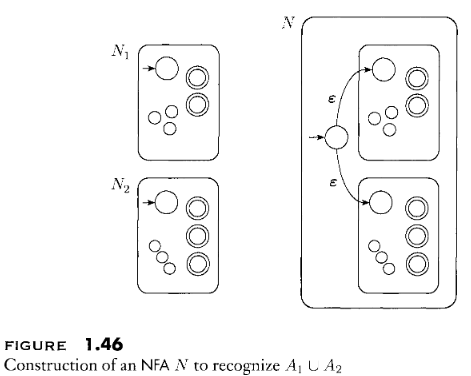
\includegraphics[scale=.5]{Q4-SipserAutom}

\problem*{5}
\question{Complete a prova do Teorema 6, mostrando que $L(C) = A B$ (formalizando a ideia que vimos em aula).}

	$Resp:$ Da página 60 do Sipser (teorema 1.46) a classe das linguagens regulares é fechada sob concatenação.
	Seja $A =(Q_A,\Sigma,\delta_A,q_A,F_A)$ e $B = (Q_B,\Sigma,\delta_B,q_B,F_B)$.\\
	Construimos $C = (Q,\Sigma,\delta,q_A,F_B)$ para reconhecer $AB$.
	\begin{enumerate}
		\item $Q = Q_A \cup Q_B$, os estados de $C$ são todos os estados de $A$ mais os de $B$;
		\item O estado $q_A$ é o estado inicial de $C$;
		\item Os estados de aceitação de $C$ são $F_B$, os mesmos de $B$. 
		\item Definimos $\delta$ para quaisqueres $q \in Q$ e $a \in \Sigma$:\\
		$\delta(q,a) = \begin{cases}
							\delta_A(q,a),\qquad q \in Q_A \ e \ q \notin F_A;\\
							\delta_A(q,a),\qquad q \in F_A \ e \ a \neq \lambda;\\
							\delta_A(q,a) \cup \{q_B\},\qquad q \in F_A \ e \ a = \lambda;\\
							\delta_B(q,a), \qquad  q \in Q_B.
					   \end{cases}					  
		$
	\end{enumerate}
	Como conseguimos construir um autômato finito $C$ que reconhece concatenção de autômatos finitos, temos que $L(C) = L(AB)$ é regular.
	Figura do livro:\\
	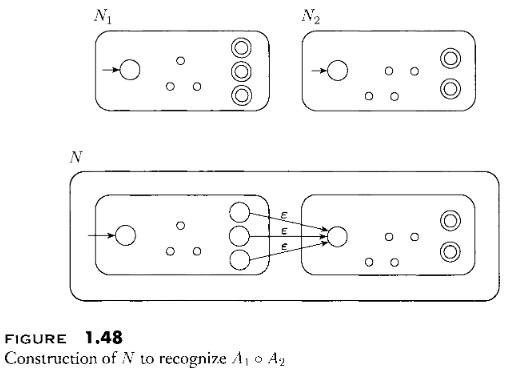
\includegraphics[scale=.5]{Q5-SipserAutom}
\end{document}
